\section{Eternity II}
	\subsection{Les origines}
	--- [réel]
	
	EternityII est le fier successeur de Eternity.
	
	La première version [image](photo de la première version), sortie en 1999, était composée de 159 pièces de différentes formes, cependant ces formes peuvent être décomposés en formes de trianges equilatéraux (ou leur moitié) qui devaient être placés sur un plateau octogonal. 
	
	\begin{figure}[H]
		\minipage{0.65\textwidth}
		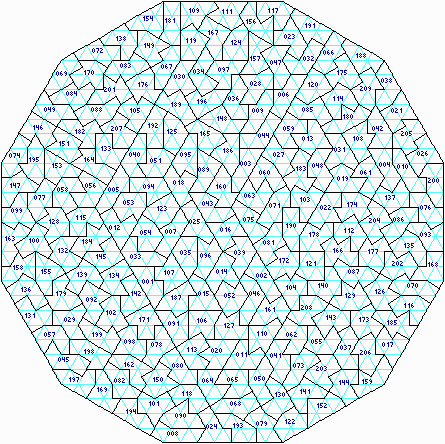
\includegraphics[width=\linewidth]{images/eternity_1.jpg}
		\caption{Eternity I}\label{fig:eternity_1}
		\endminipage\hfill
		\minipage{0.33\textwidth}
		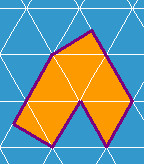
\includegraphics[width=\linewidth]{images/eternity_1_piece.jpg}
		\caption{Forme d'une pièce d'EternityI}\label{fig:eternity_1_piece}
		\endminipage\hfill
	\end{figure}

	Son point faible se trouvaient dans la disposition de ces pièces sur le plateau : il était possible de précalculer des régions, puis de les comparer entre eux afin d'en dégager une solution.
	De cette facon, le puzzle fut résolu en à peine un an (contrairement aux 3 ans prévus par le créateur), par deux mathématiciens, qui ont ainsi empoché la récompense s'élevant à $1000000\pounds$.
	
	Après cet \enquote{echec}, Christopher Monckton, le créateur d'Eternity, décide en 2008 de sortir une deuxième version, bien plus complexe avec à la clé $2000000\textdollar$ pour celui qui arriverait à la résoudre au bout de deux ans.
	
	\begin{figure}[H]
		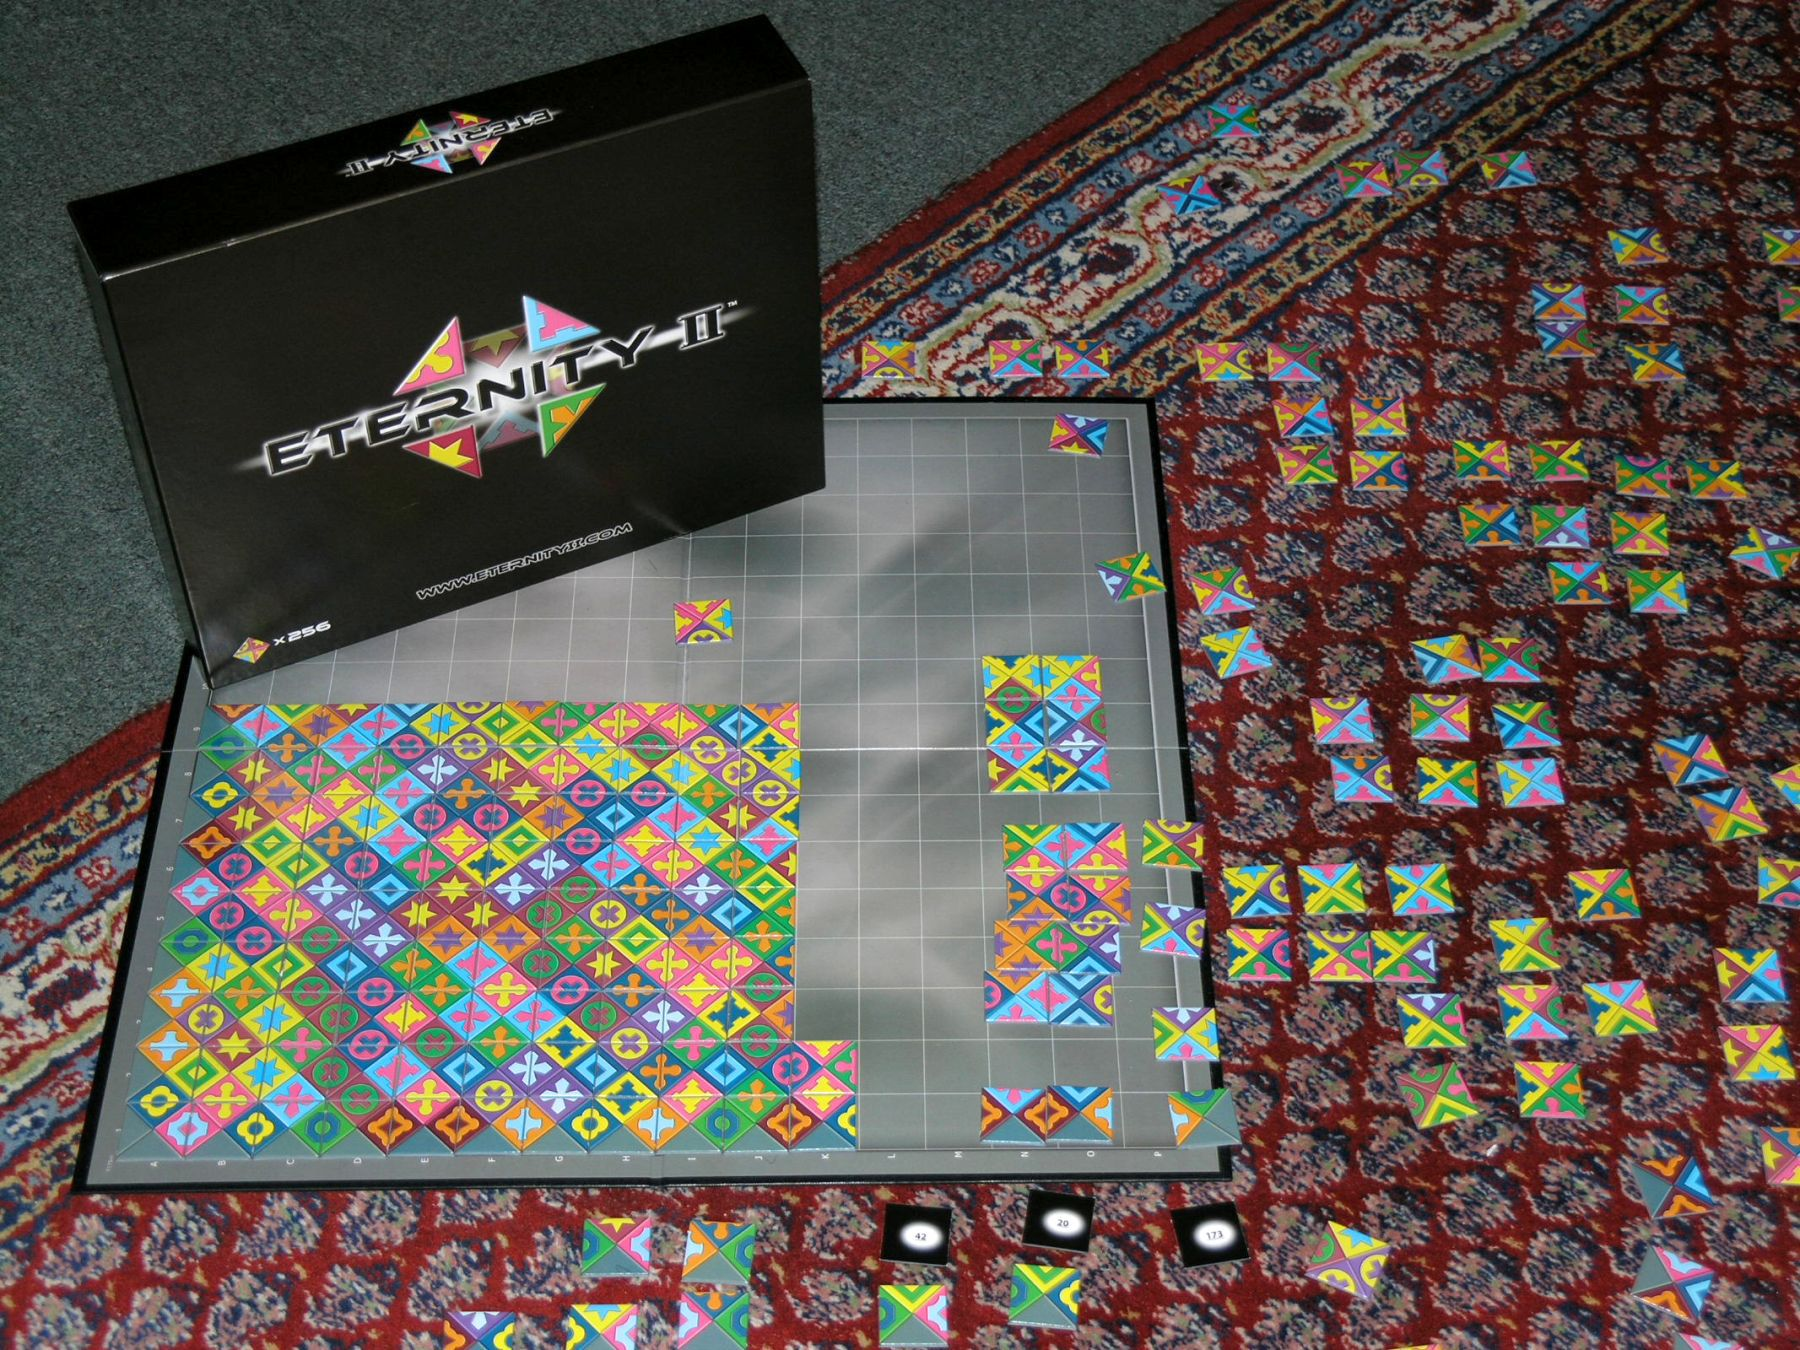
\includegraphics[width=\linewidth]{images/eternity_2.jpg}
		\caption{La boite et les pièces d'EternityII}
		\label{fig:eternity_2}
	\end{figure}
	
	C'est un puzzle de 16 par 16 qui sort sous le nom d'EternityII. Ce puzzle est composé de 256 pièces carrés, qui ont chacune 4 faces colorés (ou un demi motif).
	
	Ces pièces peuvent être classés en trois catégories suivant le nombre de faces grises qu'elles possèdent :
	
	\begin{figure}[H]
	   	\minipage{0.32\textwidth}
	   	
\includegraphics[width=\linewidth]{images/piece_coin.png}
	   	\caption{\textbf{pièce de coin :} 2 faces grises}\label{fig:piece_coin}
	   	\endminipage\hfill
	   	\minipage{0.32\textwidth}
	   	
\includegraphics[width=\linewidth]{images/piece_bord.png}
	   	\caption{\textbf{pièce de bord :} 1 faces grise}\label{fig:piece_bord}
	   	\endminipage\hfill
	   	\minipage{0.32\textwidth}
	   	
\includegraphics[width=\linewidth]{images/piece_interieure.png}
	   	\caption{\textbf{pièce d'intérieur :} toutes les faces de couleur}\label{fig:piece_interieure}
	   	\endminipage
	\end{figure}

	Les pièces ne possèdent pas de formes comme dans un puzzle classique. Afin de les faire correspondre l'une avec l'autre, il est nécessaire que les faces adjacentes de chaque pièce voisine soient de la même couleur. Par conséquent, la pièce peut être placée n'importe ou sur le plateau car son placement dépends des couleurs des pièces d'à côté, de plus, les pièces n'ont pas d'orientation prédéterminés (elle peut être rotationnée).
	
	Pour résumer, la plupart des pièces peuvent être posés n'importe où sur le plateau à différentes rotation car la position dépends entièrement des pièces adjacentes posés auparavant. 
	
	Enfin, comme leur nom l'indiquent, les pièces de coins sont les seules à pouvoir être posés dans les coins du plateau, c'est aussi valable pour les pièces de bord qui ne peuvent être placés que sur les bords du plateau.
	
	
	--- [résumé]
	
	Eternity II est un jeu sorti en 2008 qui repose sur un principe assez simple, c'est un puzzle de 16 par 16 qu'il faut réassembler. Il est composé de 256 pièces carrés, qui ont, sur chaque arête une couleur donnée. [images tt ca tt ca]. Afin de pouvoir assembler le puzzle, il suffit placer les pièces de façon à ce que les faces adjacentes soient de même couleur. Comme un puzzle classique, il y a des pièces de coin et de bord. Ceux-ci sont reconnaissables car ils possèdent une ou deux arêtes grises. Par contre, la où ca devient complexe, c'est qu'une pièce n'as pas une place prédéterminée (comme dans un puzzle), c'est à dire qu'elle peux se situer n'importe où sur le plateau. 
	
	\subsection{Le défi}
	--- [réel]
	
	Malgré le fait que la récompense à expiré le 31 décembre de l'année 2010, le problème et l'enthousiasme qu'a engendré EternityII ne s'est pas calmé pour autant (enfin si, un peu). Car loin d'être juste un jeu avec une importante cagnotte il recel en son c\oe ur des secrets d'une certaine valeur.
	
	En effet, jusqu'à maintenant, personne n'a réussi à résoudre ce puzzle, même pas effleuré la solution, malgré l'aide de supercalculateurs et de nombreux spécialistes, que ce soient des mathématiciens ou des informaticiens.
	
	Pourquoi ? Car derrière ce jeu anodin se cache l'un des plus grand problème du monde actuel : les problèmes NP-difficiles. Ceux-ci sont fait de telle sorte que même ne connaissant leur structure ou fonctionnement, il est pratiquement impossible d'en déduire un algorithme (moyen de résoudre) afin de trouver la solution. Ce type de problème est communément appliqué dans le chiffrement. Car le meilleur moyen de cacher une aiguille (solution) est de la cacher dans gros paquet d'aiguilles, plus le tas est gros, plus on met de temps à la [l'aiguille] trouver.
	
	\begin{exmp}
		Le nombre de combinaisons possibles pour Eternity II s'élève à $10^{545}$, c'est à dire environ $10^{450}$ fois le nombre d'atomes dans l'univers connu (estimé à au plus $10^{80}$) !!! Ca fait un gros tas d'aiguilles !!
	\end{exmp}
		
	--- [résumé]
	
	A ce jour, personne n'a réussi à résoudre ce puzzle (même grâce à l'aide de supercalculateurs) malgré les différentes stratégies mise en place. Pourquoi ? Car derrière ce jeu anodin se cache l'un des plus grand problème du monde actuel : les problèmes NP-difficiles. Ceux-ci sont fait de tel sorte que même en connaissant leur structure ou fonctionnement, il est pratiquement impossible d'en déduire un algorithme de résolution. L'une des solutions les plus fiables à ce jour est de tester tout les cas possible (qui est évidemment très important).
	
	\begin{exmp}
		Le nombre de combinaisons pour Eternity II s'élève à $10^{545}$, c'est à dire environ $10^{450}$ fois le nombre d'atomes dans l'univers connu (estimé à au plus $10^{80}$) !!!
	\end{exmp}
	
	\subsection{La recette secrète d'Eternity II}
	
	Pour rendre ce problème combinatoire, il est nécessaire de respecter plusieurs conditions.
	
	\begin{description}
		\item[Chaque pièce est unique] l'unicité des pièces est importante, car si une pièce est en double, cela veux dire que la pièce peux être placée à deux endroits différents (ce qui simplifie le problème)
		\item[Le ratio de nombre de couleurs par nombre de pièces est calculé] [joindre graphique tt ca tt ca] : il faut qu'il y ait assez de couleur pour que chaque pièce soit unique, mais pas assez pour que l'on puisse déterminer les pièces adjacentes
		
		\begin{exmp}
			Supposons qu'il y ait trop de couleurs. Cela veux dire qu'une pièce à peu de voisins ( car chaque pièce est unique, par conséquent les couleurs sont distribués uniformément à travers les pièces), si la pièce à très peu de voisins, je peux déduire des groupement de pièces assez facilement.
			
			Donc je simplifie mon problème.
		\end{exmp}		
	\end{description}
	
	\subsection{Etat de l'art}
	
	Nombreux sont ceux qui ont essayé de résoudre le problème... plusieurs moyens ont été mis en place, grâce au solveur SAT (solveur de satisfiabilité booléenne dont le fonctionnement est assez complexe pour ne pas être abordé ici), par une approche graphe ou encore par bruteforce.
	
	Il est estimé que actuellement, l'approche la plus performante est la résolution par bruteforce, car c'est elle qui est la plus rapide.
	
	[à développer]